\documentclass[a4paper,oneside,12pt, extrafontsizes]{memoir}

\usepackage{graphicx}
\usepackage{verbatim}
\usepackage{amsthm}

\theoremstyle{definition}
\newtheorem*{examples}{Examples}

\theoremstyle{definition}
\newtheorem*{concrete-syntax}{Concrete Syntax}

\theoremstyle{definition}
\newtheorem*{abstract-syntax}{Abstract Syntax}

\theoremstyle{definition}
\newtheorem*{constraints}{Constraints}

\renewcommand{\rmdefault}{ppl}
\chapterstyle{demo2}
\renewcommand\partnumberlinebox[2]{#2\hspace{1em}}
\renewcommand\chapternumberlinebox[2]{#2\hspace{1em}}

\usepackage{hyperref}
\hypersetup{pdftex,colorlinks=true,allcolors=blue}
\usepackage{hypcap}

\usepackage{color}
\definecolor{dark_blue}{rgb}{0.0,0.0,0.7}
\definecolor{fielddrab}{rgb}{0.42, 0.33, 0.12}

\usepackage{textcomp}
\usepackage{listings}
\lstset{upquote=true,basicstyle=\footnotesize,frame=single}
\lstdefinelanguage{cml}
{
  identifierstyle=\color{dark_blue},
  morestring=[b]",
  stringstyle=\color{fielddrab},
  morecomment=[l]{--},
  commentstyle = \color{black},
  morekeywords={,abstract,concept,task,association,select,reject,
  yield,recurse,count,first,last,if,then,else,for,in,}
}
\lstdefinelanguage{antlr}
{
  identifierstyle=\color{dark_blue},
  morestring=[b]",
  stringstyle=\color{fielddrab},
  morekeywords={,returns,}
}
\lstdefinelanguage{lsl}
{
  identifierstyle=\color{dark_blue},
  morestring=[b]',
  stringstyle=\color{fielddrab},
  morecomment=[l]{//},
  commentstyle = \color{black},
  morekeywords={,node,select,reject,
  yield,recurse,count,first,last,if,then,else,for,in,}
}
\lstdefinelanguage{ocl_}
{
  identifierstyle=\color{dark_blue},
  morestring=[b]',
  stringstyle=\color{fielddrab},
  morecomment=[l]{--},
  commentstyle = \color{black},
  morekeywords={,self,context,def,inv,pre,post,and,or,implies,derive,body,if,then,else,}
}

\title{\emph{Conceptual Modeling Language}\\Specification\\ \small{Version 1.0 (Draft)}}
\author{Quenio Cesar Machado dos Santos\\
\small{Universidade Federal de Santa Catarina}\thanks{
Initially developed as part of the author's Bachelor Technical Report in Computer Sciences}}
\date{July 2017}

\makeatletter
\newcommand{\verbatimfont}[1]{\renewcommand{\verbatim@font}{\ttfamily#1}}
\makeatother

\makeatletter
\renewcommand*{\p@chapter}{\S\,}
\renewcommand*{\p@section}{\S\,}
\renewcommand*{\p@subsection}{\S\,}
\makeatother

\begin{document}

\begin{titlingpage}
\maketitle
\end{titlingpage}

\frontmatter

\begin{KeepFromToc}

\clearpage
\tableofcontents

\clearpage
\listoffigures

\clearpage
\listoftables

\end{KeepFromToc}

\mainmatter

\part{Language and Compiler}

\chapter{The Language}
This document specifies the \emph{Conceptual Modeling Language}, or CML for short.
CML enables the modeling of the information of software systems.
It focuses on modeling the structural aspects of such systems,
having less emphasis on the behavioral aspects.
Using CML,
it is possible to represent the information as understood by the system users,
while disregarding its physical organization as implemented by target languages or technologies.

In this first part of the CML specification,
the first chapter will provide an overview of the CML compiler's architecture,
and the second chapter describes the organization and notation
used in the remainder of this document.
The second part describes that structural constructs of the language
that enable conceptual modeling.
The third part focuses on the semantics of type checking.
The fourth part covers values and expressions.
The fifth part describes code generation.
The last part will cover organization and sharing of conceptual models.


\chapter{The Compiler}
\label{ch:compiler}
The CML compiler has as \emph{input},
source files defined using its own conceptual language (as specified in this document),
which provides an abstract syntax similar to (but less comprehensive than) a combination of UML \cite{uml} and OCL \cite{ocl};
and, as \emph{output}, any target languages based on extensible templates,
which may be provided by the compiler's base libraries, by third-party libraries, or even by developers.

\begin{figure}
\centering
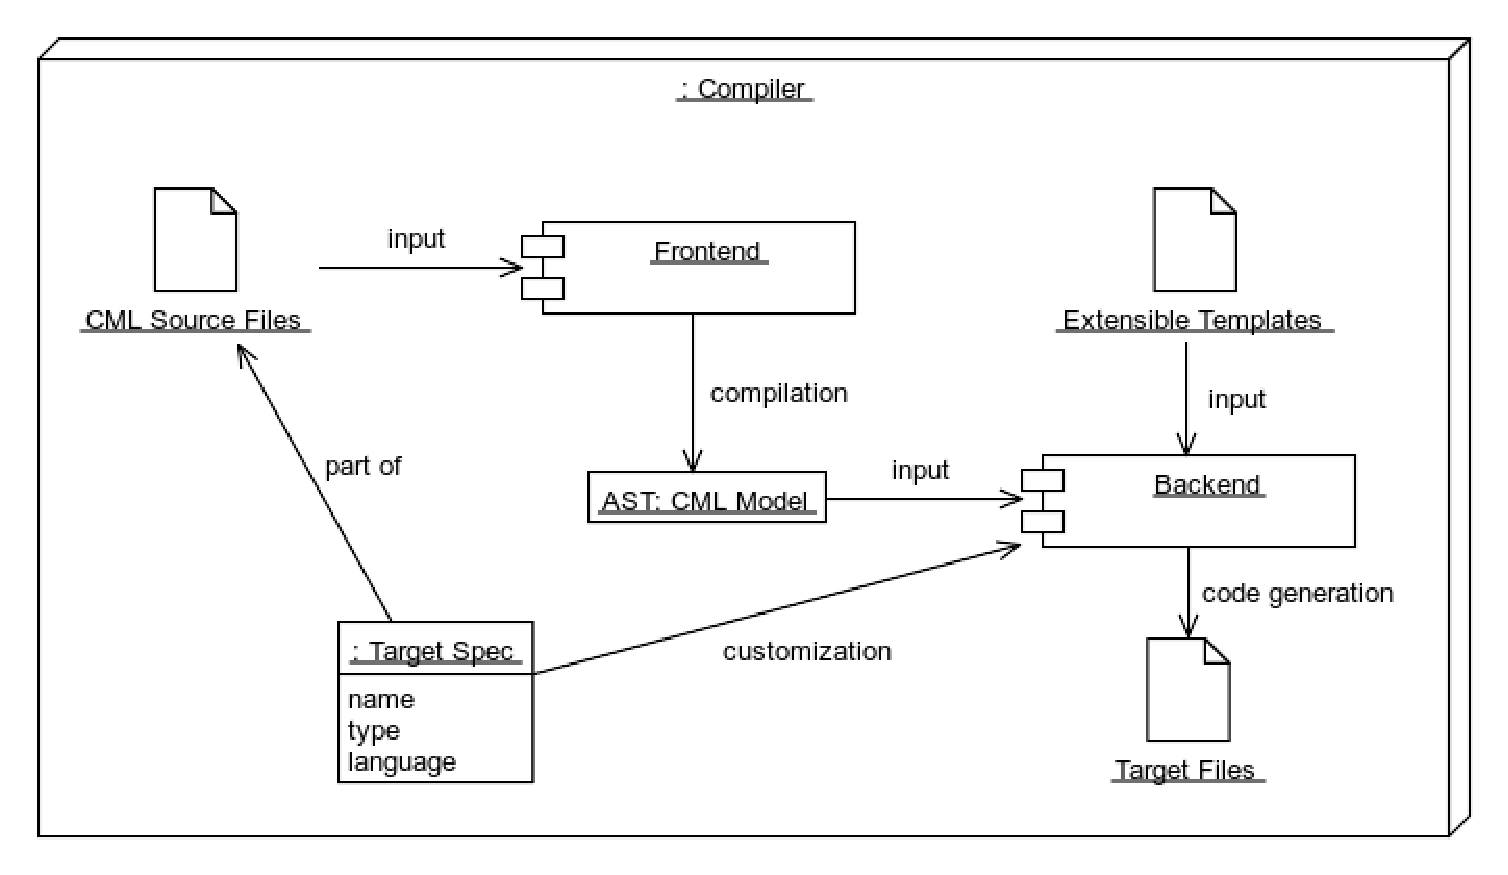
\includegraphics[width=\textwidth]{compiler/figure-overview}
\caption{An architectural overview of the CML compiler.}
\label{fig:overview}
\end{figure}

The CML compiler's overall architecture follows the standard compiler design literature \cite{torben}. An overview diagram of the architecture is shown in figure \ref{fig:overview}.
The two main components of the compiler,
and the artifacts they work with,
are presented in the next subsections.


\section[The Frontend]{The Compiler Frontend}
\label{sec:frontend}
The frontend receives as input the \emph{CML source files}.
It will parse the files and generate an internal representation of the \emph{CML model}.

Syntactical and semantic validations will be performed at this point.
Any syntax and constraint errors are presented to the developer, interrupting the progress to the next phase.
If the \emph{source files} are parsed and validated successfully, then the internal representation (the AST) of the \emph{CML model} is provided as the input for the \emph{backend} component.


\section[The Backend]{The Compiler Backend}
\label{sec:backend}
The backend receives the \emph{CML model AST} as input.
Based on the \emph{target specification} provided by the AST, chooses which \emph{extensible templates} to use for code generation.
The \emph{target files} are then generated, and become available to be consumed by other tools. The \emph{task declaration} plays the key role of determining the kind of \emph{target} to be generated.

CML extensible templates are implemented in StringTemplate \cite{st}.  The CML compiler uses StringTemplate for two purposes:

\begin{itemize}
\item \emph{File names and directory structure:}
each type of target generated by the CML compiler requires a different directory structure.
The CML compiler expects each target type to define a template file named ``files.stg'' (also known as \emph{files template}),
which will contain the path of all files to be generated. The \emph{files template} may use information provided by the \emph{task declaration}
in order to determine the file/directory names.
\item \emph{File content generation:}
each file listed under the \emph{files template} will have a corresponding \emph{content template} that specifies how the file's content must be generated. The \emph{content template} will receive as input one root-level element of the CML model, which will provide information to generate the file's content.
Each type of top-level model element should have a corresponding \emph{content template}. Templates are described in \emph{Code Generation} part of this specification.
\end{itemize}


\chapter{Specification and Notations}
\label{ch:notations}
The following chapters will specify every element of CML metamodel.
Each chapter starts with a definition, followed by: an example;
the specification of the concrete syntax;
and then presenting the abstract syntax,
and how to transform the concrete syntax into the abstract one.

Chapters may also have sections that specify sub-elements
of the top-level CML metamodel element being described in the chapter level.
Each sub-element is described under its section
using the same definition structure (detailed below)
that is used to define the top-level elements.

The definition of each CML metamodel element is stated in plain English
on a paraprah (such as this one)
starting with the ``\textbf{Definition.}'' heading.
If a correspondence exists to an element of
the Entity-Relationship (ER) \cite{er} metamodel,
or to an element of the Unified Modeling Language (UML) \cite{uml} metamodel,
it is provided.

\begin{examples}
For each metamodel element declaration in CML,
examples are provided on a paraprah (such as this one),
starting with the ``\textbf{Examples.}'' heading.
This type of paragraph refers to a \verb+verbatim+ figure
containing the examples, and describes them as needed.
The examples are provided for illustrative purposes only,
and they are \emph{not} intended to be normative.
They may be excerpts of larger CML source files,
and thus may not be successfully compiled on their own.
\end{examples}

\begin{concrete-syntax}
The concrete syntax of each CML metamodel element is described
on a paragraph (such as this one),
starting with the ``\textbf{Concrete Syntax.}'' heading.
This type of paragraph refers to a \verb+verbatim+ figure,
which contains the actual ANTLR \cite{antlr} grammar
specifying the syntax for the CML metamodel element in question,
and it must be considered normative.
The appendix \ref{apx:concrete-syntax} presents all the grammar rules
in a single listing.
\end{concrete-syntax}

\begin{abstract-syntax}
The abstract syntax of each CML metamodel element is described
on a paragraph (such as this one),
starting with the ``\textbf{Abstract Syntax.}'' heading.
This type of paragraph refers to two types of figure:
the first figure presents a class diagram
with the EMOF \cite{mof}-based metamodel
of the element being described;
the second figure specifies the transformation
from the concrete syntax into instances of the metamodel classes,
which are the nodes of the abstract syntax tree
(the intermediate representation described in section \ref{sec:compiler}).
The notation used to specify the transformations is presented
in the appendix \ref{apx:lsl}.
Both figures must be considered normative.
\end{abstract-syntax}

\begin{constraints}
The constraints of each CML metamodel element are described
on a paragraph (such as this one),
starting with the ``\textbf{Constraints.}'' heading.
This type of paragraph refers to a \verb+verbatim+ figure,
which contains the OCL \cite{ocl} invariants
(and its definitions)
of the CML metamodel element in question,
and it must be considered normative.
Each invariant has a name in the format \verb+inv_name+
so that it can be referred by the compiler's error messages
and users.
Derived properties may also be defined before the constraints
in order to simplify the constraint expressions.
The appendix \ref{apx:ocl} presents all the constraint rules
in a single listing.
\end{constraints}

All metamodel elements referred by one of the descriptions defined above
(definitions, examples, etc.)
are emphasized in \emph{italic}.
If the descriptions of a CML metamodel element refer to another CML metamodel element,
the corresponding chapter or section defining the other element
is provided in parenthesis, like so (\ref{sec:org}).

Some sections may not follow the structure defined above.
These normally provide additional semantic information in plain English,
which cannot be described using the notations presented above.


\part{Conceptual Modeling}

\chapter{Concepts}
\label{ch:concepts}
A \emph{concept} in CML represents anything
that has a coherent, cohesive and relevant meaning in a domain.
In the ER \cite{er} metamodel,
it corresponds to an \emph{entity set} (or an \emph{entity type});
in UML \cite{uml},
to a \emph{class}.
The CML \emph{concept} differs, however, from the UML \emph{class},
because it has only \emph{properties} (\ref{sec:properties}),
while the UML \emph{class} may also have \emph{operations}.

\begin{examples}
Figure \ref{fig:ex:concepts} presents some examples of \emph{concepts} declared in CML.
As shown,
a \emph{concept} may have zero or more \emph{properties}
(\ref{sec:properties}),
and a \emph{property} may optionally declare a \emph{type}
(\ref{sec:primitive-types}, \ref{sec:collection-types}).
Also, as shown in the concept \textbf{EBook} of the example,
a \emph{concept} may specialize
(\ref{sec:generalization})
another \emph{concept}.
\end{examples}

\begin{figure}
\verbatimfont{\small}
\lstinputlisting[language=cml]{examples/concepts.cml}
\caption{Concept Examples}
\label{fig:ex:concepts}
\end{figure}

\begin{concrete-syntax}
Figure \ref{fig:stx:concept} specifies the syntax used
to declare a \emph{concept}.
The \textbf{concept} keyword is followed by a NAME.
Optionally, a list of other NAMEs may be enumerated,
referring to other \emph{concepts}
that are generalizations (\ref{sec:generalization}) of the declared \emph{concept}.
A list of \emph{properties} (\ref{sec:properties}) may be declared under the \textbf{concept} block.
And the \textbf{abstract} keyword may precede the \textbf{concept} keyword, making a \emph{concept} abstract (\ref{sec:abstract}).
\end{concrete-syntax}

\begin{figure}
\verbatimfont{\small}
\lstinputlisting[language=antlr]{grammar/Concepts.txt}
\caption{Concept Declaration Syntax}
\label{fig:stx:concept}
\end{figure}

\begin{abstract-syntax}
Figure \ref{fig:meta:concept} presents the \emph{concept} metamodel
in an EMOF \cite{mof} class diagram,
and figure \ref{fig:ast:concept} specifies
the \emph{concept} transformation
from its concrete syntax to its abstract syntax.
For each \emph{concept} parsed by the compiler,
an instance of the \emph{Concept} class will be created,
and its properties will be assigned
according to parsed information:

\begin{itemize}

\item \emph{name}:
assigned with the value of the terminal node NAME.

\item \emph{abstract}:
set to \emph{true} if the \textbf{abstract} keyword
is found before the \textbf{concept} keyword;
otherwise, set to \emph{false}.

\item \emph{elements}:
an \emph{ordered set} referencing all \emph{properties}
parsed in the \textbf{concept} block.

\item \emph{generalizations}:
an \emph{ordered set} referencing all \emph{concepts}
whose NAMEs were enumerated in the \emph{GeneralizationList}.

\end{itemize}
\end{abstract-syntax}

\begin{figure}
\centering
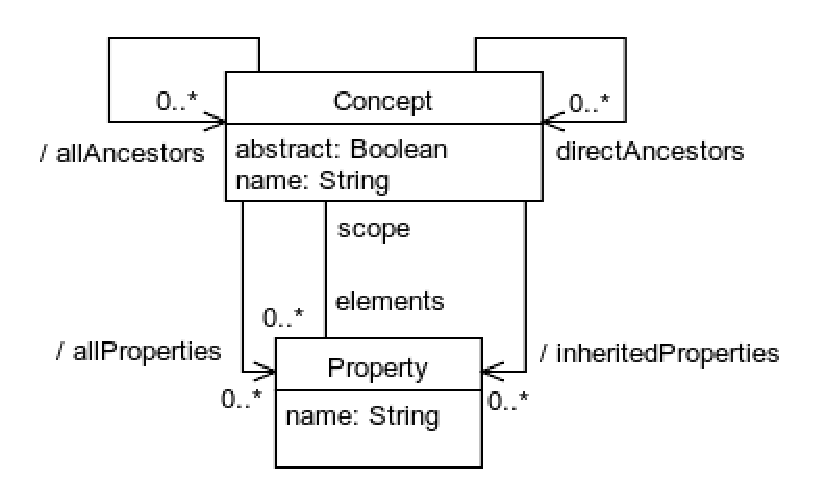
\includegraphics[width=0.5\textwidth]{metamodel/concept}
\caption{Concept Metamodel}
\label{fig:meta:concept}
\end{figure}

\begin{figure}
\verbatimfont{\small}
\lstinputlisting[language=lsl]{ast/concept.lsl}
\caption{Concept AST Instantiation}
\label{fig:ast:concept}
\end{figure}

\begin{constraints}
Figure \ref{fig:ocl:concept} presents the invariants of the \emph{concept} metamodel:

\begin{itemize}

\item \emph{unique\_concept\_name}:
Each \emph{concept} must have a unique NAME within its \emph{module} (\ref{ch:modules}).

\end{itemize}
\end{constraints}

\begin{figure}
\lstinputlisting[language=ocl_]{ocl/concept.ocl}
\caption{Concept Constraints}
\label{fig:ocl:concept}
\end{figure}


\chapter{Properties}
\label{ch:properties}
A \emph{property} in CML may hold \emph{values} of \emph{primitive types} (\ref{ch:primitive-types}),
in which case they correspond to \emph{attributes} (\ref{ch:attributes})
on the ER \cite{er} and UML \cite{uml} metamodels.
Or they may hold references, or \emph{sequences} of references (\ref{ch:sequence-types}),
linking to instances of other \emph{concepts} (\ref{ch:concepts}),
in which case they correspond to a \emph{relationship} on the ER metamodel,
or to \emph{associations} (\ref{ch:associations}) on the UML metamodel.


\chapter{Attributes}
\label{ch:attributes}
In CML, \emph{attributes} are \emph{properties} (\ref{ch:properties})
of \emph{primitive types} (\ref{ch:primitive-types}).
They correspond to the \emph{Attribute} metaclass
in the ER \cite{er} metamodel;
in the UML \cite{uml} metamodel,
to the association \emph{attribute} between the metaclass \emph{Class}
and the metaclass \emph{Property}.

\emph{Attributes} serve as a \emph{slot} that holds a value of
the specified \emph{primitive type}.
An initial value may be specified as an \emph{expression} (\ref{ch:expressions}).
Some \emph{attributes}, however, may be continuosly
derive their \emph{value} from an \emph{expression} (not only initially),
in which case they are called \emph{derived attributes} (\ref{ch:derived-attributes}).

While initial values are only set when a \emph{concept} (\ref{ch:concepts})
is instantiated,
the value of \emph{derived attributes} is always evaluated
from the given \emph{expression},
and they cannot be set any other way.


\chapter{Derived Attributes}
\label{ch:derived-attributes}
A \emph{concept} in CML may have \emph{attributes} (\ref{ch:attributes})
that do not hold specific \emph{values},
but instead provide a \emph{value} derived from an \emph{expression} (\ref{ch:expressions}).
These are called \emph{derived attributes}.
Unlike an \emph{expression} used to initialize a \emph{non-derived attribute},
the \emph{expression} of a \emph{derived attribute} is evaluated
every time the \emph{value} of an \emph{attribute} is fetched.

In the UML \cite{uml} metamodel,
the \emph{Property} metaclass has a meta-attribute named \emph{isDerived},
which determines whether an \emph{attribute} is derived or not.
A \emph{derived attribute} in UML may be defined using a OCL \cite{ocl} constraint;
while CML has \emph{expressions} as part of the language.

The ER \cite{er} metamodel,
in its original form,
does not allow for the differentiation of \emph{derived attributes}
as part of an \emph{entity set},
but it is possible to define \emph{retrieval operations} whose 
results would equal to \emph{values} of \emph{derived properties} in CML.
It can be said, however, that ER,
by defining an \emph{attribute} as a function from the \emph{entity set}
to the \emph{value set},
does not prescribe that all \emph{attributes} are memory-based,
nor does it prevent the definition of an \emph{attribute} function 
as an \emph{expression}.

The CML metamodel and its syntax, on the other hand,
define whether an \emph{attribute} is memory-based (a \emph{non-derived attribute})
or it is derived from an \emph{expression} (a \emph{derived attribute}).


\section{Derived Attributes - Example}
Figure \ref{fig:ex:attributes} presents two examples of \emph{derived attributes}
declared in CML.
As shown,
the attribute \textbf{c} is derived from an \emph{expression}
that refers to other \emph{attributes}.
In order to differentiate \emph{attributes} with initial values,
such as \textbf{b},
from \emph{derived attributes},
such as \textbf{c},
a forward slash (``/'') prefixes the name of the latter.
The attribute \textbf{e} is an example of a \emph{derived attribute}
where the type is inferred from the given \emph{expression},
instead of being specified.


\section{Derived Attributes - Syntax}
Figure \ref{fig:stx:property} specifies the syntax used
to declare any kind of \emph{property} (\ref{ch:properties}),
including \emph{derived attributes}.
A \emph{derived attribute} must be prefixed with the forward-slash character,
as specified by DERIVED,
in which case the given \emph{expression} provides the value
of the \emph{attribute} every time it is fetched.

The \emph{property} metaclass in the CML metamodel is used to represent
\emph{attributes}.
Figure \ref{fig:meta:property} presents the \emph{property} metaclass
in an EMOF \cite{mof} class diagram,
and figure \ref{fig:ast:property} specifies
the \emph{property} transformation
from its concrete syntax to its abstract syntax.
The \emph{derived} property of the \emph{Property} metaclass
defines whether the \emph{attribute} is derived or not.


\chapter{Associations}
\label{ch:associations}
In CML,
an \emph{association} represents a relation between two \emph{concepts} (\ref{ch:concepts}),
where a reference to an \emph{instance} of each \emph{concept} is found in every tuple that is part of the relation.
When \emph{concepts} have an \emph{association},
its \emph{instances} are linked in such way that
it is possible to access an \emph{instance} of one \emph{concept}
from an \emph{instance} of the other \emph{concept}.

The UML \cite{uml} metamodel has a metaclass named \emph{Association} that has \emph{Property} instances,
whose \emph{types} are the \emph{Class} instances that are part of the \emph{association}.
In UML, the name of each \emph{Property} instance in the \emph{Association} metaclass
is known as the \emph{role} of the corresponding \emph{Class} in the \emph{association}.

On the CML metamodel, on other hand,
the \emph{Association} metaclass is only needed
when it is necessary to define \emph{bidirectional associations}.
For \emph{unidirectional associations},
only a \emph{property} is defined in the source \emph{concept},
making its \emph{type} the target \emph{concept}.

On the ER \cite{er} metamodel,
each \emph{association} is known as a \emph{relationship set},
and each tuple in this set is called a \emph{relationship}.
Unlike CML and UML,
the tuples in a \emph{relationship set} of an ER model
can be queried directly,
and no notion of \emph{property} is required as part of the \emph{entity type}
in order to access those \emph{relationships}.

As it is case for \emph{attributes} (\ref{ch:attributes}),
\emph{associations} in CML can also be derived from other \emph{associations}
(just as well as in UML);
they are called \emph{derived associations} (\ref{sec:derived-associations}).

\begin{examples}
Figure \ref{fig:ex:associations} presents some examples of \emph{associations} declared in CML.
The concept \textbf{Vehicle} contains the property \textbf{driver},
which may optionally refer to an instance of \textbf{Employee},
meaning that a \textbf{driver} may or may not be assigned to a single \textbf{Vehicle}.
The concept \textbf{Vehicle} also has the property \textbf{owner},
which always refers to an instance of \textbf{Organization},
meaning that an \textbf{owner} must always be assigned to each instance of \textbf{Vehicle}. 
Similarly,
the concept \textbf{Employee} has the property \textbf{employer},
which must always be assigned to instance of \textbf{Organization}.
Just below the declaration of \textbf{Organization},
we observe an association named \textbf{Employment},
which enumerates two \emph{properties}:
the first is \textbf{employer} from the concept \textbf{Employee};
the second is \textbf{employees} from the concept \textbf{Organization}.
What this \emph{association} implies is a correspondence between these two properties.
Every time a reference to an instance of \textbf{Organization} is assigned to
the slot \textbf{employer} of an instance of \textbf{Employee},
a reference to this same instance of \textbf{Employee} must be assigned to
the slot \textbf{employees} of the \textbf{Organization} instance.
However,
since the \emph{type} of \textbf{employees}
in the concept \textbf{Organization}
is a sequence of \textbf{Employee} instances,
the reference to the instance of \textbf{Employee} will actually be added to the sequence,
along with the other instances already found in the sequence.
Thus, the association \textbf{Employment} actually characterizes a \emph{bidirectional association}.
The association \textbf{VehicleOwnership} is another example of a \emph{bidirectional association};
in this case,
between \textbf{Vehicle}'s \textbf{owner} property and \textbf{Organization}'s \textbf{fleet} property.
It can be noticed, though, 
in this second \emph{bidirectional association},
that the \emph{types} of the \emph{properties} are declared along with their names;
such a \emph{type} declaration,
in the \emph{association} declaration,
is optional in CML,
but must match the original \emph{property} declaration under the \emph{concept} declaration,
if present.
The \textbf{driver} property in the concept \textbf{Vehicle} is a different case,
since this \emph{property} does not participate in any \emph{association} declaration
in figure \ref{fig:ex:associations}.
That's because there is no corresponding \emph{property} in the concept \textbf{Employee}
representing the other end of the \emph{association}.
As such, the property \textbf{driver} is representing the source end of a \emph{unidirectional association}.
The property \textbf{drivers} in the concept \textbf{Organization} will be explained
in the section \ref{sec:derived-associations}.
\end{examples}

\begin{figure}
\verbatimfont{\small}
\lstinputlisting[language=cml]{examples/associations.cml}
\caption{Association Examples}
\label{fig:ex:associations}
\end{figure}

\begin{concrete-syntax}
Figure \ref{fig:stx:association} specifies the syntax used
to declare an \emph{association}.
The \textbf{association} keyword is followed by a NAME.
A list of \emph{association ends} are declared under the \textbf{association} block.
For each declaration of an \emph{association end},
The \textbf{conceptName} and \textbf{propertyName} are optionally followed by a \emph{typeDeclaration}.
\end{concrete-syntax}

\begin{figure}
\verbatimfont{\small}
\lstinputlisting[language=antlr]{grammar/Associations.txt}
\caption{Association Declaration Syntax}
\label{fig:stx:association}
\end{figure}

\begin{abstract-syntax}
Figure \ref{fig:meta:association} presents the \emph{Association} metaclass
in an EMOF \cite{mof} class diagram,
and figure \ref{fig:ast:association} specifies
the \emph{association} transformation
from its concrete syntax to its abstract syntax.
For each \emph{association} parsed by the compiler,
an instance of the \emph{Association} class will be created,
and its properties will be assigned
according to parsed information:

\begin{itemize}

\item \emph{name}:
assigned with the value of the terminal node NAME.

\item \emph{members}:
an \emph{ordered set} referencing all \emph{associationEnd}
instances parsed in the \textbf{association} block.

\end{itemize}
\end{abstract-syntax}

\begin{figure}
\verbatimfont{\small}
\lstinputlisting[language=lsl]{ast/association.lsl}
\caption{Association AST Instantiation}
\label{fig:ast:association}
\end{figure}

\begin{constraints}

\end{constraints}

\section{Associations - Example}
Listing \ref{lst:ex:associations} presents some examples of \emph{associations} declared in CML.
The concept \textbf{Vehicle} contains the property \textbf{driver},
which may optionally refer to an instance of \textbf{Employee},
meaning that a \textbf{driver} may or may not be assigned to a single \textbf{Vehicle}.
The concept \textbf{Vehicle} also has the property \textbf{owner},
which always refers to an instance of \textbf{Organization},
meaning that an \textbf{owner} must always be assigned to each instance of \textbf{Vehicle}.
Similarly,
the concept \textbf{Employee} has the property \textbf{employer},
which must always be assigned to an instance of \textbf{Organization}.

Just below the declaration of \textbf{Organization},
we observe an association named \textbf{Employment},
which enumerates two \emph{properties}:
the first is \textbf{employer} from the concept \textbf{Employee};
the second is \textbf{employees} from the concept \textbf{Organization}.
What this \emph{association} implies is a correspondence between these two properties.
Every time a reference to an instance of \textbf{Organization} is assigned to
the slot \textbf{employer} of an instance of \textbf{Employee},
a reference to this same instance of \textbf{Employee} must be assigned to
the slot \textbf{employees} of the \textbf{Organization} instance.
However,
since the \emph{type} of \textbf{employees}
in the concept \textbf{Organization}
is a sequence of \textbf{Employee} instances,
the reference to the instance of \textbf{Employee} will actually be appended to the sequence
being held by the slot \textbf{employees} of the concept \textbf{Organization},
and maintained along with the other \textbf{Employee} instances already found in the sequence.
Thus, the association \textbf{Employment} actually characterizes a \emph{bidirectional association}.

The association \textbf{VehicleOwnership} is another example of a \emph{bidirectional association};
in this case,
between \textbf{Vehicle}'s \textbf{owner} property and \textbf{Organization}'s \textbf{fleet} property.
It can be noticed, though,
in this second \emph{bidirectional association},
that the \emph{types} of the \emph{properties} are declared along with their names;
such a \emph{type} declaration,
in the \emph{association} declaration,
is optional in CML,
but must match the original \emph{property} declaration under the \emph{concept} declaration,
if present.

The \textbf{driver} property in the concept \textbf{Vehicle} is a different case,
since this \emph{property} does not participate in any \emph{association} declaration
on listing \ref{lst:ex:associations}.
That's because there is no corresponding \emph{property} in the concept \textbf{Employee}
representing the other end of the \emph{association}.
As such, the property \textbf{driver} is representing the source end of a \emph{unidirectional association}.

The property \textbf{drivers} in the concept \textbf{Organization}
is \emph{derived association} (\ref{ch:derived-associations}).

\begin{code}
\verbatimfont{\small}
\lstinputlisting[language=cml]{examples/associations.cml}
\caption{Association Example}
\label{lst:ex:associations}
\end{code}


\section{Associations - Syntax}
The concrete syntax used to declare an \emph{association} in CML
is specified by listing \ref{lst:stx:association}.
First, the \textbf{association} keyword is followed by a NAME.
Then, a list of \emph{association ends} are declared under the \textbf{association} block.
For each declaration of an \emph{association end},
The \textbf{conceptName} and \textbf{propertyName} are optionally followed by a \textbf{typeDeclaration}.

\begin{code}
\verbatimfont{\small}
\lstinputlisting[language=antlr]{grammar/Associations.txt}
\caption{Association Concrete Syntax}
\label{lst:stx:association}
\end{code}

The \emph{Association} metaclass is presented 
in the EMOF \cite{mof} class diagram of figure \ref{fig:meta:associations},
and its instantiation from the concrete syntax is specified by listing \ref{lst:ast:associations}.
For each parsed \emph{association},
an instance of the \emph{Association} metaclass will be created,
and its meta-properties will be assigned
according to parsed information:

\begin{itemize}

\item \emph{name}:
assigned with the value of the token NAME.

\item \emph{members}:
an \emph{ordered set} referencing all \emph{associationEnd}
instances parsed in the \textbf{association} block.

\end{itemize}

\begin{code}
\verbatimfont{\small}
\lstinputlisting[language=lsl]{ast/associations.lsl}
\caption{Association AST Instantiation}
\label{lst:ast:associations}
\end{code}


\section{Associations - Constraints}
The invariants of the metaclasses \emph{Association} and \emph{AssociationEnd}
are specified by listing \ref{lst:inv:associations}:

\begin{itemize}

\item \emph{association\_end\_property\_found\_in\_model}:
Each \emph{association end} enumerated under an \emph{association}
must correspond to a \emph{property} of the same name under the specified \emph{concept}.

\item \emph{association\_end\_type\_matches\_property\_type}:
If a \emph{type} is specified for a given \emph{association end},
its \emph{name} and \emph{cardinality} must match the \emph{type}
of the corresponding \emph{property}.

\item \emph{association\_must\_have\_two\_association\_ends}:
An \emph{association} must have exaclty two \emph{association ends},
since only \emph{binary associations} are supported in CML.

\item \emph{association\_end\_types\_must\_match}:
The \emph{concept} of one \emph{association end} must correspond
to the \emph{type} of the \emph{property} of the other \emph{association end},
and vice-versa.

\end{itemize}

\begin{code}
\lstinputlisting[language=ocl_]{constraints/associations.ocl}
\caption{Association Constraints}
\label{lst:inv:associations}
\end{code}



\chapter{Derived Associations}
\label{ch:derived-associations}

\chapter{Generalization / Specialization}
\label{ch:generalization}
A \emph{concept} (\ref{ch:concepts}) in CML may be generalized by another \emph{concept}.
In other words, a \emph{concept} may be considered a specialization of another \emph{concept}.
Generalized \emph{concepts} have \emph{properties} (\ref{sec:properties})
that apply to a larger set of instances,
while specialized \emph{concepts} have \emph{properties}
that only apply to a subset of those instances.

In the UML \cite{uml} metamodel,
such generalization/specialization relationship between \emph{classes}
is known as \emph{generalization}, which is the name of the metaclass in the UML metamodel.
The original version of the ER \cite{er} metamodel lacked this kind of relationship
between \emph{entity types}.


\chapter{Abstract Concepts}
\label{ch:abstract}
An \emph{abstract concept} is one that does not represent specific instances,
but instead serves as a \emph{generalization} (\ref{ch:generalization}) 
for other \emph{concepts},
which in turn represent specific instances.
Thus, all instances of an \emph{abstract concept}
are first instances of its \emph{specializations}.
CML supports tagging a \emph{concept} as \emph{abstract}.

An \emph{abstract concept} in CML may also define a \emph{derived property} (\ref{sec:properties})
wihtout providing an \emph{expression} (\ref{ch:expressions}) in its definition;
such \emph{properties} may also be called \emph{abstract properties}.

CML's support for \emph{abstract concepts} matches UML's \cite{uml},
which allows the declaration of \emph{abstract classes}
-- by setting the \emph{isAbstract} attribute of the \emph{Class} metaclass instance to \emph{true}.
UML also allows the declaration of corresponding \emph{abstract attributes} and \emph{abstract operations}.

The original version of the ER \cite{er} metamodel, however,
as a consequence of lacking the \emph{generalization/specialization} relationship,
has not considered the notion of \emph{abstract entities}.

\begin{examples}
Figure \ref{fig:ex:abstract} presents an example of an \emph{abstract concept} declared in CML.
As shown, the concept \textbf{Shape} is tagged as \emph{abstract},
and as such no direct instances of \emph{Shape} are ever instantiated.
As an \emph{abstract concept}, \textbf{Shape} can define \emph{abstract properties},
like \textbf{area}, which is just a \emph{derived property} (\ref{sec:properties})
without an \emph{expression} (\ref{ch:expressions}).
An \emph{abstract concept} may also define concrete \emph{properties},
such as \textbf{color} in \textbf{Shape}.
The concept \textbf{Circle} is a \emph{especialization} of \textbf{Shape}
that must redefine the property \textbf{area}
(and provide an \emph{expression})
if it is to be considered a \emph{concrete concept}.
As a \emph{concrete concept},
\textbf{Circle} may have direct instances,
which are in turn instances of \emph{Shape} as well.
\textbf{Circle} may also redefine \emph{concrete properties} of \textbf{Shape},
like \textbf{color},
but the redefinition is not a requirement in this case.
In \textbf{UnitCircle},
we can observe that the redefinition of an \emph{abstract property},
such as \textbf{area},
may be made \emph{concrete};
meaning it does not need to be redefined as a \emph{derived property}.
The converse situation is also allowed in CML,
where a \emph{concrete property} is redefined by as a \emph{derived property},
as illustrated with the property \textbf{radius} in \textbf{UnitCircle}.
\end{examples}

\begin{figure}
\verbatimfont{\small}
\lstinputlisting[language=cml]{examples/abstract.cml}
\caption{Abstract Concept Example}
\label{fig:ex:abstract}
\end{figure}

\begin{concrete-syntax}
Figure \ref{fig:stx:concept} specifies the syntax used
to declare a \emph{concept} (\ref{ch:concepts}) in CML.
It shows that a \emph{concept} may be tagged with the \textbf{abstract} keyword
in order to convey it as an \emph{abstract concept}.
Figure \ref{fig:stx:property} specifies the syntax used 
to declare a \emph{property} (\ref{sec:properties}) in CML.
It shows that a \emph{property} may be prefixed with a forward slash (``/'')
in order to mark it as a \emph{derived property}.
If the optional \textbf{expression} is not provided,
the property is then considered an \emph{abstract property}.
\end{concrete-syntax}

\begin{abstract-syntax}
Figure \ref{fig:meta:concept} presents the \emph{concept} metamodel
in an EMOF \cite{mof} class diagram,
and figure \ref{fig:ast:concept} specifies
the \emph{concept} transformation
from its concrete syntax to its abstract syntax.
There is a \textbf{Boolean} attribute named \textbf{abstract} in the \emph{Concept} class
that determines whether a \emph{concept} is \emph{abstract} or not.
\end{abstract-syntax}

\begin{constraints}
Figure \ref{fig:ocl:abstract} presents the invariants
of the \emph{Concept} and \emph{Property} classes in CML's EMOF \cite{mof} metamodel
related to \emph{abstract concepts}:

\begin{itemize}

\item \emph{abstract\_property\_redefinition}:
A \emph{concrete concept} must redefine concretely all \emph{abstract properties} of 
its \emph{generalizations}.

\item \emph{abstract\_property\_in\_abstract\_concept}:
Only \emph{abstract concepts} may have \emph{abstract properties}.

\end{itemize}
\end{constraints}

\begin{figure}
\lstinputlisting[language=ocl_]{ocl/abstract.ocl}
\caption{Abstract Concept Constraints}
\label{fig:ocl:abstract}
\end{figure}



\section{Abstract Concepts - Example}
Listing \ref{lst:ex:abstract} presents an example of an \emph{abstract concept} declared in CML.
As shown, the concept \textbf{Shape} is tagged as \emph{abstract},
and as such no direct instances of \emph{Shape} are ever instantiated.
As an \emph{abstract concept}, \textbf{Shape} can define \emph{abstract properties},
like \textbf{area}, which is just a \emph{derived property} (\ref{ch:properties})
without an \emph{expression} (\ref{ch:expressions}).
An \emph{abstract concept} may also define concrete \emph{properties},
such as \textbf{color} in \textbf{Shape}.
The concept \textbf{Circle} is a \emph{especialization} of \textbf{Shape}
that must redefine the property \textbf{area}
(and provide an \emph{expression})
if it is to be considered a \emph{concrete concept}.
As a \emph{concrete concept},
\textbf{Circle} may have direct instances,
which are in turn instances of \emph{Shape} as well.
\textbf{Circle} may also redefine \emph{concrete properties} of \textbf{Shape},
like \textbf{color},
but the redefinition is not a requirement in this case.
In \textbf{UnitCircle},
we can observe that the redefinition of an \emph{abstract property},
such as \textbf{area},
may be made \emph{concrete};
meaning it does not need to be redefined as a \emph{derived property}.
The converse situation is also allowed in CML,
where a \emph{concrete property} is redefined by as a \emph{derived property},
as illustrated with the property \textbf{radius} in \textbf{UnitCircle}.

\begin{code}
\verbatimfont{\small}
\lstinputlisting[language=cml]{examples/abstract.cml}
\caption{Abstract Concept Example}
\label{lst:ex:abstract}
\end{code}



\section{Abstract Concepts - Syntax}
Listing \ref{lst:stx:concept} specifies the syntax used
to declare a \emph{concept} (\ref{ch:concepts}) in CML.
It shows that a \emph{concept} may be tagged with the \textbf{abstract} keyword
in order to convey it as an \emph{abstract concept}.
Listing \ref{lst:stx:property} specifies the syntax used
to declare a \emph{property} (\ref{ch:properties}) in CML.
It shows that a \emph{property} may be prefixed with a forward slash (``/'')
in order to mark it as a \emph{derived property}.
If the optional \textbf{expression} is not provided,
the property is then considered an \emph{abstract property}.

Figure \ref{fig:meta:concept} presents the \emph{concept} metamodel
in an EMOF \cite{mof} class diagram,
and listing \ref{lst:ast:concept} specifies
the \emph{concept} transformation
from its concrete syntax to its abstract syntax.
There is a \textbf{Boolean} attribute named \textbf{abstract} in the \emph{Concept} class
that determines whether a \emph{concept} is \emph{abstract} or not.


\section{Abstract Concepts - Constraints}
Figure \ref{fig:ocl:abstract} presents the invariants
of the \emph{Concept} and \emph{Property} classes in CML's EMOF \cite{mof} metamodel
related to \emph{abstract concepts}:

\begin{itemize}

\item \emph{abstract\_property\_redefinition}:
A \emph{concrete concept} must redefine concretely all \emph{abstract properties} of 
its \emph{generalizations}.

\item \emph{abstract\_property\_in\_abstract\_concept}:
Only \emph{abstract concepts} may have \emph{abstract properties}.

\end{itemize}

\begin{figure}
\lstinputlisting[language=ocl_]{ocl/abstract.ocl}
\caption{Abstract Concept Constraints}
\label{fig:ocl:abstract}
\end{figure}


\part{Type System}

\chapter{Types}

\chapter{Primitive Types}
\label{ch:primitive-types}
A \emph{primitive type} in CML is one of the pre-defined \emph{data types}
supported by the language,
as shown in tables \ref{tab:core-primitive-types} and \ref{tab:additional-primitive-types}.

In the ER \cite{er} metamodel,
a \emph{data type} is formally defined as a \emph{set} of \emph{values}
that can be held by an \emph{attribute} (\ref{ch:attributes}).
The original ER paper \cite{er} states that,
for each \emph{value set} (i.e. \emph{data type}),
there is a \emph{predicate} that can be used to test
whether a \emph{value} belongs to the \emph{set}.
In CML, instead,
\emph{literal expressions} are syntactically defined for each \emph{primitive type},
so that the \emph{type} can be inferred from the \emph{literal expression}.

On the original ER paper,
it is also said that \emph{values} in a \emph{value set}
may be equivalent to \emph{values} in another \emph{value set}.
In CML, also,
\emph{literal expressions} of the \emph{Integer} type may be equivalent
to \emph{literal expressions} of the \emph{Decimal},
and so with other \emph{numeric types}.
This allows \emph{expressions} (\ref{ch:expressions}) of a \emph{primitive type}
to be promoted to \emph{expressions} of another \emph{primitive type}
in order to allow \emph{type inference} of composite \emph{expressions}.

In the UML \cite{uml} metamodel,
there is a specific metaclass named \emph{PrimitiveType},
which matches to the same notion in CML.

\begin{table}[h]
\centering
\begin{tabular}
{l l l l l p{2cm} }
\hline
CML & Java & C\# & C++ & Python & TypeScript (JavaScript) \\
\hline
String & String & string & std::wstring & str & string \\
\multicolumn{6}{p{13cm}}{\footnotesize{16-bit Unicode character sequences.}} \\
\\
Boolean & boolean & bool & bool & bool & boolean \\
\multicolumn{6}{p{13cm}}{\footnotesize{Only values are the literal expressions: \textbf{true}, \textbf{false}.}}  \\
\\
Integer & int & int & int32\_t & int & number  \\
\multicolumn{6}{p{13cm}}{\footnotesize{32-bit signed two's complement integer.}}  \\
\\
Decimal* & BigDecimal & decimal & decimal128 & Decimal & number \\
\multicolumn{6}{p{13cm}}{\footnotesize{Arbitrary precision,
fixed-point,
or decimal floating-point,
depending on the target language.}} \\
\\
\multicolumn{6}{p{13cm}}{*The specification of Decimal type varies by target programming language.
Compared to the binary floating-point types (Float and Double),
the Decimal type is better suited for monetary calculations
at a performance cost.}
\end{tabular}
\caption{Core Primitive Types in CML.}
\label{tab:core-primitive-types}
\end{table}

\begin{table}[h]
\centering
\begin{tabular}
{l l l l l p{2cm} p{3.5cm} }
\hline
CML & Java & C\# & C++ & Python & TypeScript (JavaScript) & Specification \\
\hline
Byte & byte & byte & int8\_t & int & number & 8-bit signed two's complement integer \\
Short & short & short & int16\_t & int & number & 16-bit signed two's complement integer \\
Long & long & long & int64\_t & long & number & 64-bit signed two's complement integer \\
Float & float & float & float* & float & number & 32-bit IEEE 754 binary floating point \\
Double & double & double & double* & float & number & 64-bit IEEE 754 binary floating point \\
\\
\multicolumn{7}{p{12cm}}{*C++ floating point types may vary by hardware and compiler}
\end{tabular}
\caption{Additional Primitive Types in CML.}
\label{tab:additional-primitive-types}
\end{table}


\chapter{Sequence Types}
\label{ch:sequence-types}

\part{Values and Expressions}

\chapter{Expressions}
\label{ch:expressions}
An \emph{expression} in CML is used to compute
\emph{values} (\ref{ch:primitive-types}) and sequences (\ref{ch:sequence-types})
that initialize or derive \emph{properties} (\ref{ch:properties}).
On the UML \cite{uml} metamodel,
it corresponds to the \emph{Expression} metaclass;
in OCL \cite{ocl}, to \emph{OclExpressionCS}.

CML \emph{expressions} are designed to provide the same level of
expressivity provided by OCL \emph{expressions},
but the CML syntax varies from OCL's;
especially for OCL's \emph{collection operations},
which correspond to \emph{query expressions} (\ref{ch:queries}) in CML.



\chapter{Literal Values}
\label{ch:literals}

\chapter{Prefix Expressions}
\label{ch:prefix}

\chapter{Infix Expressions}
\label{ch:infix}

\chapter{Conditional Expressions}
\label{ch:conditionals}

\chapter{Path Expressions}
\label{ch:paths}

\chapter{Query Expressions}
\label{ch:queries}

\part{Code Generation}

\chapter{Templates}
\label{sec:templates}

\chapter{Constructors}
\label{sec:constructors}

\chapter{Tasks}
\label{sec:tasks}

\chapter{Targets}
\label{sec:targets}

\part{Organization and Sharing}

\chapter{Modules}
\label{ch:modules}

\chapter{Libraries}
\label{ch:libraries}

\part{Appendices}

\appendix

\chapter{CML Concrete Syntax (Grammar)}
\label{apx:concrete-syntax}
\clearpage
\section{ANTLR Grammar}

\begin{framed}
\verbatimfont{\small}
\begin{verbatim}
// Compilation Units:
\end{verbatim}
\verbatiminput{grammar/CompilationUnits.txt}
\begin{verbatim}
// Concept Declarations:
\end{verbatim}
\verbatiminput{grammar/Concepts.txt}
\begin{verbatim}
// Property Declarations:
\end{verbatim}
\verbatiminput{grammar/Properties.txt}
\begin{verbatim}
// Type Declarations:
\end{verbatim}
\verbatiminput{grammar/Types.txt}
\begin{verbatim}
// Target Declarations:
\end{verbatim}
\verbatiminput{grammar/Targets.txt}
\begin{verbatim}
// Names:
\end{verbatim}
\verbatiminput{grammar/Names.txt}
\begin{verbatim}
// Literals:
\end{verbatim}
\verbatiminput{grammar/Literals.txt}
\verbatiminput{grammar/Ignored.txt}
\end{framed}


\chapter{CML Abstract Syntax (Metamodel)}
\label{apx:abstract-syntax}
\input{metamodel.tex}

\chapter{CML Abstract Syntax Tree (Instantiation)}
\label{apx:ast}
\input{ast.tex}

\chapter{CML Constraints (Validations)}
\label{apx:ocl}
\clearpage

\begin{framed}
\verbatimfont{\small}
\verbatiminput{ocl/concept.ocl}
\verbatiminput{ocl/property.ocl}
\end{framed}


\chapter{Language Specification Notation}
\label{apx:lsl}
\input{lsl.tex}

\backmatter

\bibliographystyle{plain}
\bibliography{references}

\end{document}
